\chapter{引言}\label{chap:introduction}
\section{研究背景}
进入21世纪以来,网络与信息技术的发展日新月异,快速改变着人们的工作和生活方式。越来越多的政府、企业建立了依赖于网络的业务信息系统,例如电子商务、网上银行、电子政务等,对社会的各行各业造成了深远的影响。

与此同时,网络安全的重要性也在不断提升。无论是即时通信技术中的隐私保护,还是网上银行和电子商务中的财产安全,乃至信息时代中的国家安全,都离不开网络安全技术的保障。根据\cite{xintong2019zhong}发布的《中国网络安全产业白皮书》统计,2018年全球网络安全产业规模达到1119.88亿美元,预计2019年增长至1216.68亿美元。从增速上看,2018年全球网络安全产业增速为11.3\%,创下自2016年以来的新高。2014-2019年全球网络安全产业规模及增速如图1.1所示。
\begin{figure}[!htbp]
    \centering
    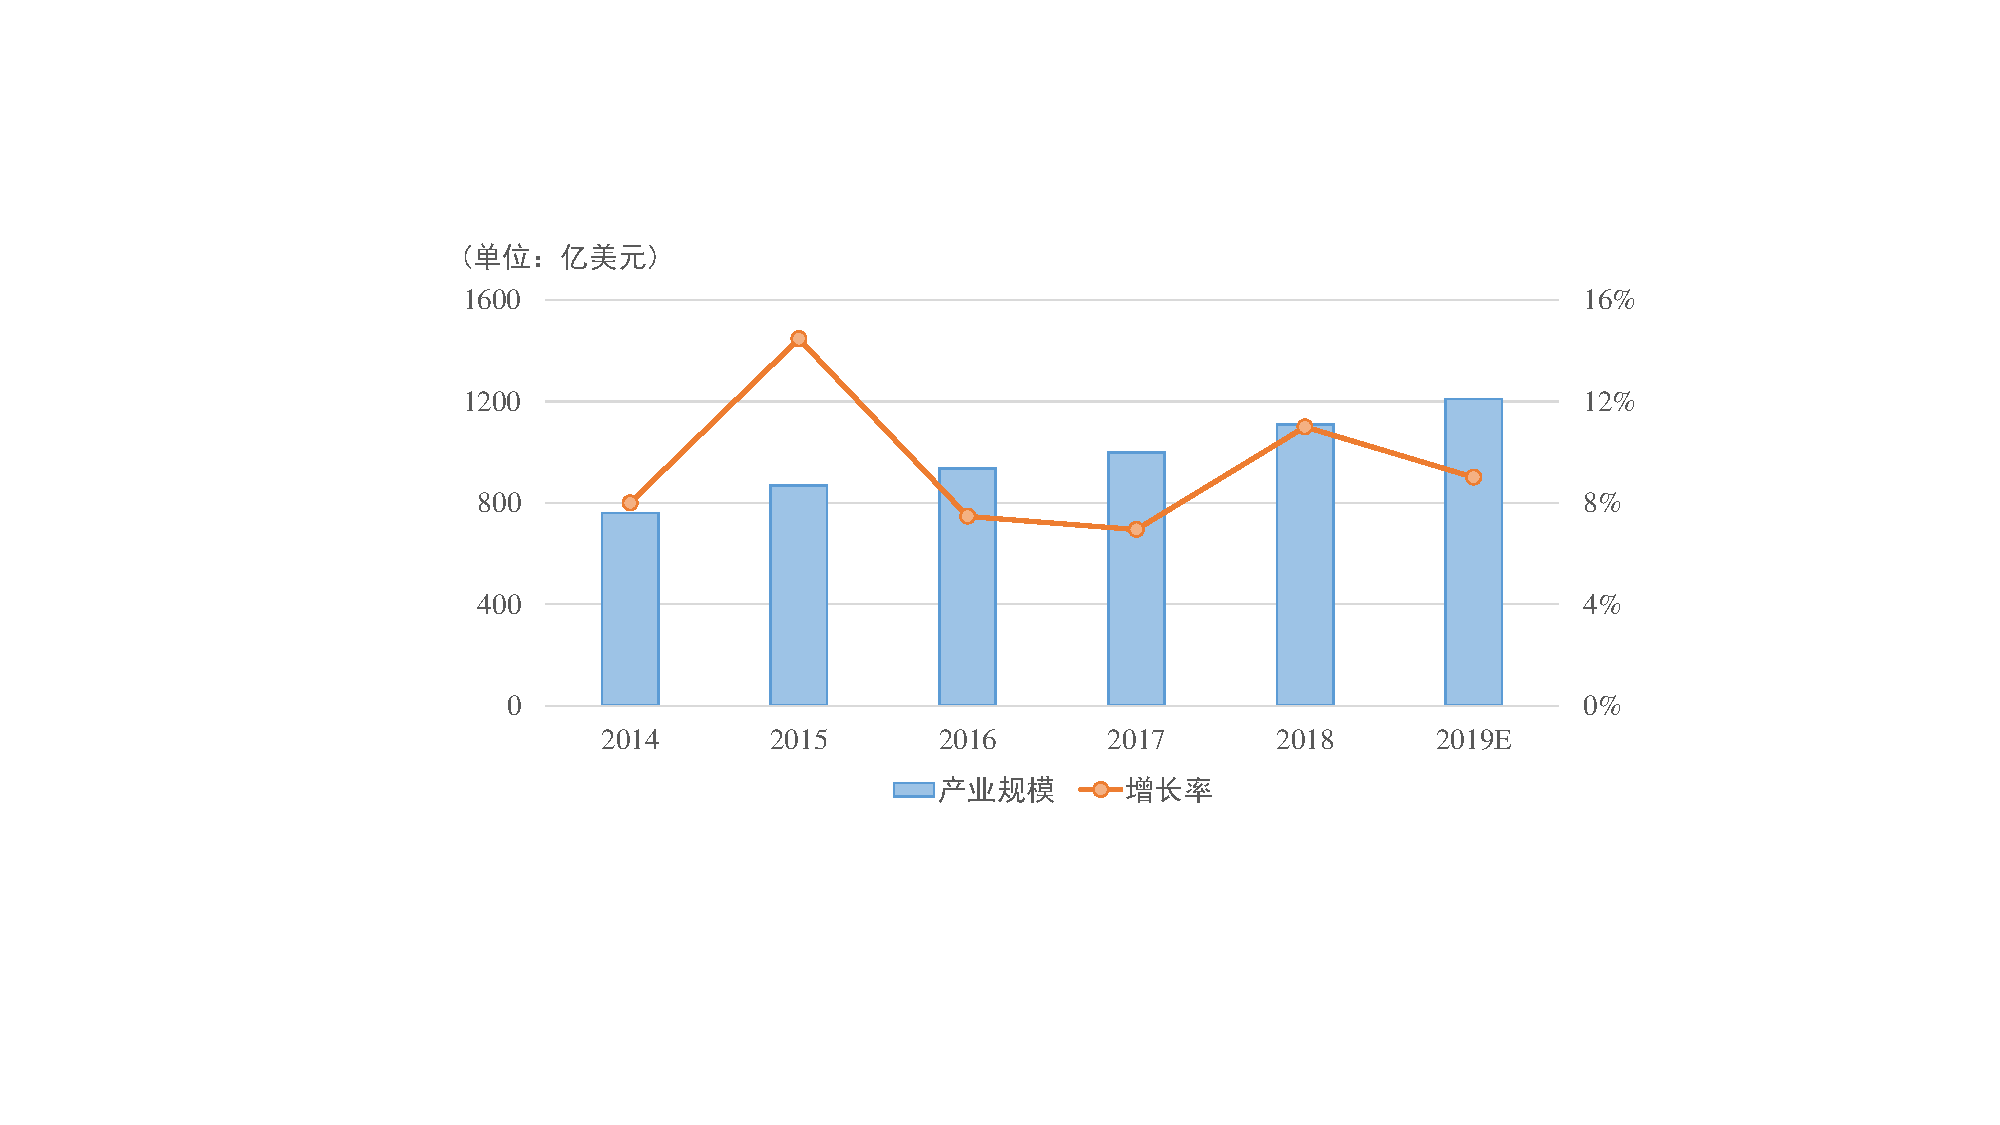
\includegraphics[width=0.9\textwidth]{网络安全产业规模及增速}
    \bicaption{2014-2019年全球网络安全产业规模及增速}{Global cyber security industry scale and growth rate, 2014-2019}
\end{figure}

此外,随着近些年互联网中移动和物联网设备数量的增多,许多企业和组织采用了日益复杂的多云架构,使得网络中的数据流不再处于传统意义上静态和高度安全的网段。同时,基于Web和移动应用的网络流量在互联网流量中的占比开始超过桌面端流量,其中大部分移动流量涉及个人敏感数据,例如支付凭证、隐私信息、社交网络等。为了适应这种变化,企业越来越依赖于利用加密手段保护数据安全,包括安全套接层(SSL)协议和传输层安全(TLS)协议。据《Google透明度报告》显示,Google产品和服务中加密流量所占比例正在平稳增长,从2014年约占48\%发展到2019年约占94\%。

\begin{figure}[!htbp]
    \centering
    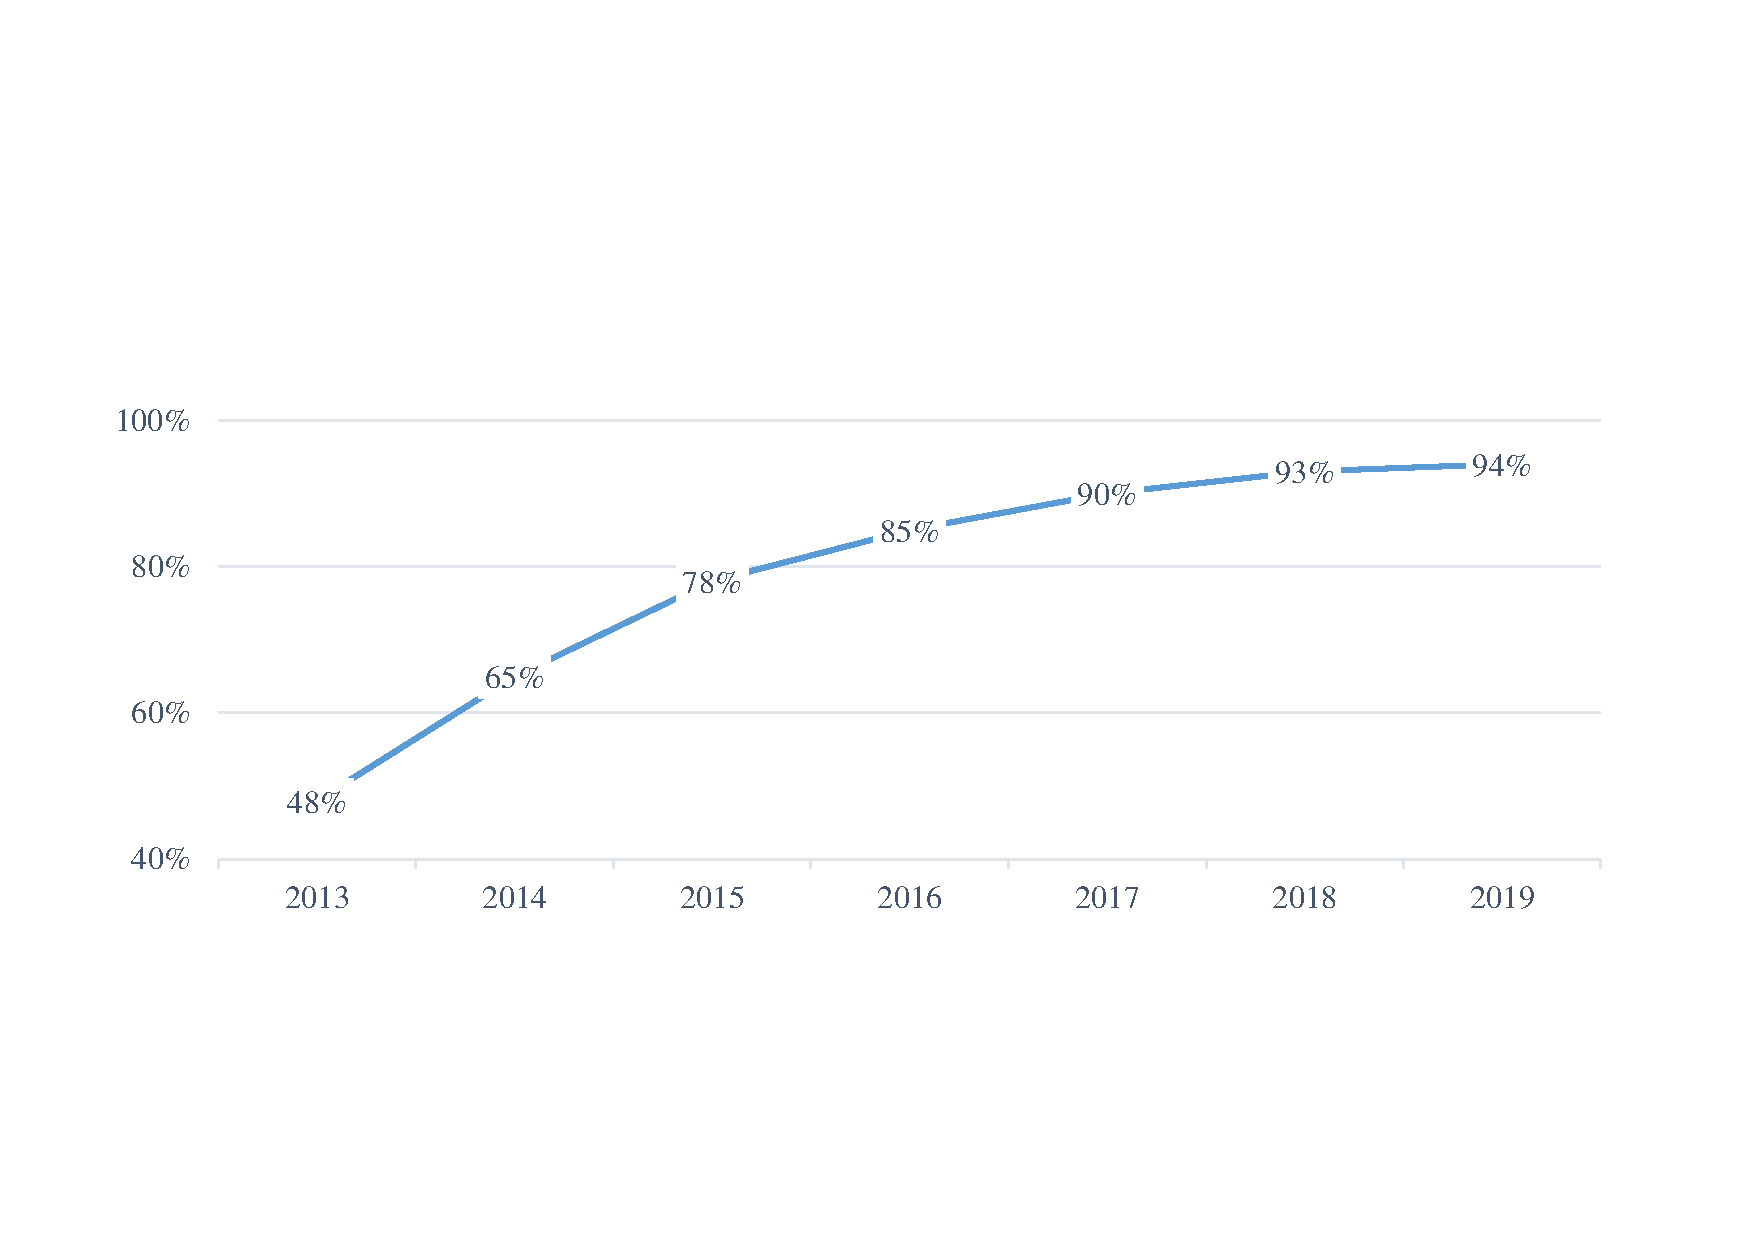
\includegraphics[width=0.9\textwidth]{1-2}
    \bicaption{2014-2019年Google产品和服务中加密流量占比增长趋势}{The growth trend of encrypted traffic in Google products and services, 2014-2019}
\end{figure}

尽管从许多方面来看,加密技术的普及对网络安全都是有利的,但同时加密流量比例的增长也对网络监管和威胁检测带来了严峻的挑战。由于加密技术只是一种工具,网络犯罪分子同样可以利用加密技术对其发起的恶意攻击进行伪装掩饰,从而逃避检测。因此,面向加密网络的流量检测技术是未来发展的必然趋势之一。

\section{研究目的和意义}

随着网络攻击行为日趋复杂,政府、企业以及个人所面临的安全威胁正在飞速增长,如蠕虫病毒、木马后门、僵尸网络、DDOS攻击等,给企业的信息网络造成严重破坏。其中,多数网络攻击的发起都与操作系统和浏览器软件漏洞有关,属于主机属性研究对象的一部分。根据\cite{guo2018zhong}发布的《中国互联网网络安全报告》显示,国家信息安全漏洞共享平台(China National Vulnerability Database, CNVD)在2018年共收录通用软硬件漏洞14201个。根据影响对象的类型,漏洞可分为:应用程序漏洞,Web应用漏洞,操作系统漏洞,网络设备漏洞,安全产品漏洞和数据库漏洞。如图1.3所示,在2018年CNVD收录的漏洞信息中,操作系统漏洞占10.6\%,Web应用漏洞占18.7\%。
\begin{figure}[!htbp]
    \centering
    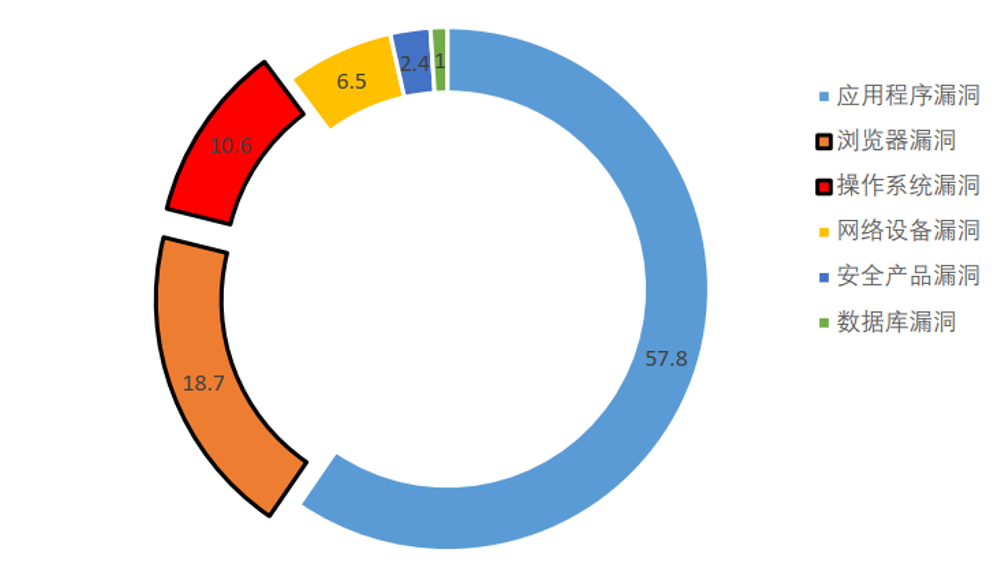
\includegraphics[width=0.8\textwidth]{1-3}
    \bicaption{2018年CNVD收录的漏洞类型分布}{Distribution of vulnerability types included in CNVD in 2018}
\end{figure}

北京时间2017年5月12日,多家安全机构监测到黑客利用美国国家安全局黑客武器库泄漏的“永恒之蓝”工具发起的网络攻击事件:大量服务器和个人电脑感染病毒后被远程控制,成为不法分子的比特币挖矿机(挖矿会耗费大量计算资源,导致机器性能降低),甚至被安装勒索软件,磁盘文件会被病毒加密为.onion或者.WNCRY后缀,用户只有支付高额赎金后才能解密恢复文件,对个人及企业的重要文件数据造成严重损失。“永恒之蓝”工具利用的是微软Windows操作系统的SMBv1协议漏洞。未经身份验证的攻击者可以向目标机器发送特制报文触发缓冲区溢出,进而在目标机器上远程执行任意代码。“永恒之蓝”工具会扫描开放445文件共享端口的Windows机器,只要用户开机上网,黑客就可能在电脑和服务器中植入勒索软件。这次攻击袭击了上百个国家不计其数的电子设备,对全球经济发展造成了难以估量的损失。

在一次完整的入侵活动中,攻击者往往采取以下几个典型步骤:信息侦察、初步入侵、系统控制、横向移动以及数据泄露等。在信息侦察阶段中,攻击者为了确定潜在目标是否满足实施入侵的条件,会利用各种技术手段对目标设备进行扫描,获取操作系统、开放端口、应用服务等信息以寻找潜在漏洞。与此相对,网络防御者可以采取安装入侵检测系统、关闭不必要的端口、提高关键设备的访问权限等手段防止攻击者获取有效信息。此外,通过研究分析攻击者侦察信息的手段,可以针对性的伪装本地主机信息,如可以通过混淆操作系统指纹使得攻击者侦察到错误信息,进而防止恶意入侵。由此可见,无论是在网络攻击还是入侵防御中,对信息的采集和识别都至关重要。一方面,攻击者需要通过目标主机信息确定下一步入侵手段,另一方面,网络管理员可以利用本地网络主机信息优化防御策略,及时修补漏洞。

综上所述,网络信息安全问题在我国以及全球日趋严重,为了国家和人民的利益,必须加强网络安全保障,提升网络安全防护能力。而信息侦察是网络攻防任务中的首要步骤,目的是为了获取目标主机的关键属性信息。因此,研究主机属性的识别技术具有十分重要的现实意义。


\section{本文的研究内容与主要贡献}

本文拟研究开放环境中的细粒度主机属性发现技术,基于加密流原始载荷的主机属性发现技术以及主机属性识别系统的设计与实现技术。本文的主要贡献包括以下三个方面:
\begin{enumerate}
    \item \textbf{开放环境中的细粒度主机属性发现。}首先以双向流流为单位,从目标主机发起的TLS会话中提取13维协议首部字段特征和3类流统计特征,包括IP协议的跳数、包长、分片标识等字段,TCP协议的传输窗口大小、窗口缩放因子、最大报文长度等字段,TLS协议的版本、扩展长度、密钥算法套件序列等字段以及流的包长序列统计特征、时间序列统计特征、速率统计特征等。然后结合以LightGBM模型为代表的机器学习算法,识别目标主机的操作系统类型、版本以及浏览器类型。
    \item \textbf{基于加密流原始载荷的主机属性发现。}随着流量数据规模的增长和机器性能的提升,深度学习模型在流量分类领域中的表现越来越出色。通过提取TLS会话中TCP SYN包和TLS Client Hello包的原始流信息,并结合以卷积神经网络模型和长短期记忆网络模型为代表的深度学习算法,可以在不需要先验知识的前提下,进一步提高开放环境中主机属性的识别精度。
    \item \textbf{主机属性识别系统的设计与实现。}本文基于Stacking技术,结合以人工特征为基础的LightGBM模型和以原始流信息为基础的深度学习模型,构建了一个用于海量主机属性发现的原型系统。该系统主要包含五个模块:流量采集模块用于在高速网络中识别并采集目标流量。特征提取模块用于从原始TLS流量中提取所需的人工特征和原始特征。属性识别模块基于Stacking技术,综合各学习模型的的检测结果,得到最终的识别信息。分类器更新模块通过对标注数据集的再学习,更新和优化属性识别模块中的分类器。数据存储与可视化模块用于识别结果的存储和可视化展示。
\end{enumerate}

\section{论文组织结构}

本文共分为六个章节,组织结构如图1.4所示。第一章是引言,第二章是国内外研究现状,第三章至第五章为本文核心内容,是对研究内容与主要贡献的详细介绍,其中第三章与第四章的研究成果又为第五章的研究内容提供技术支撑,第六章是本文研究的内容总结与未来展望。

\begin{figure}[!htbp]
    \centering
    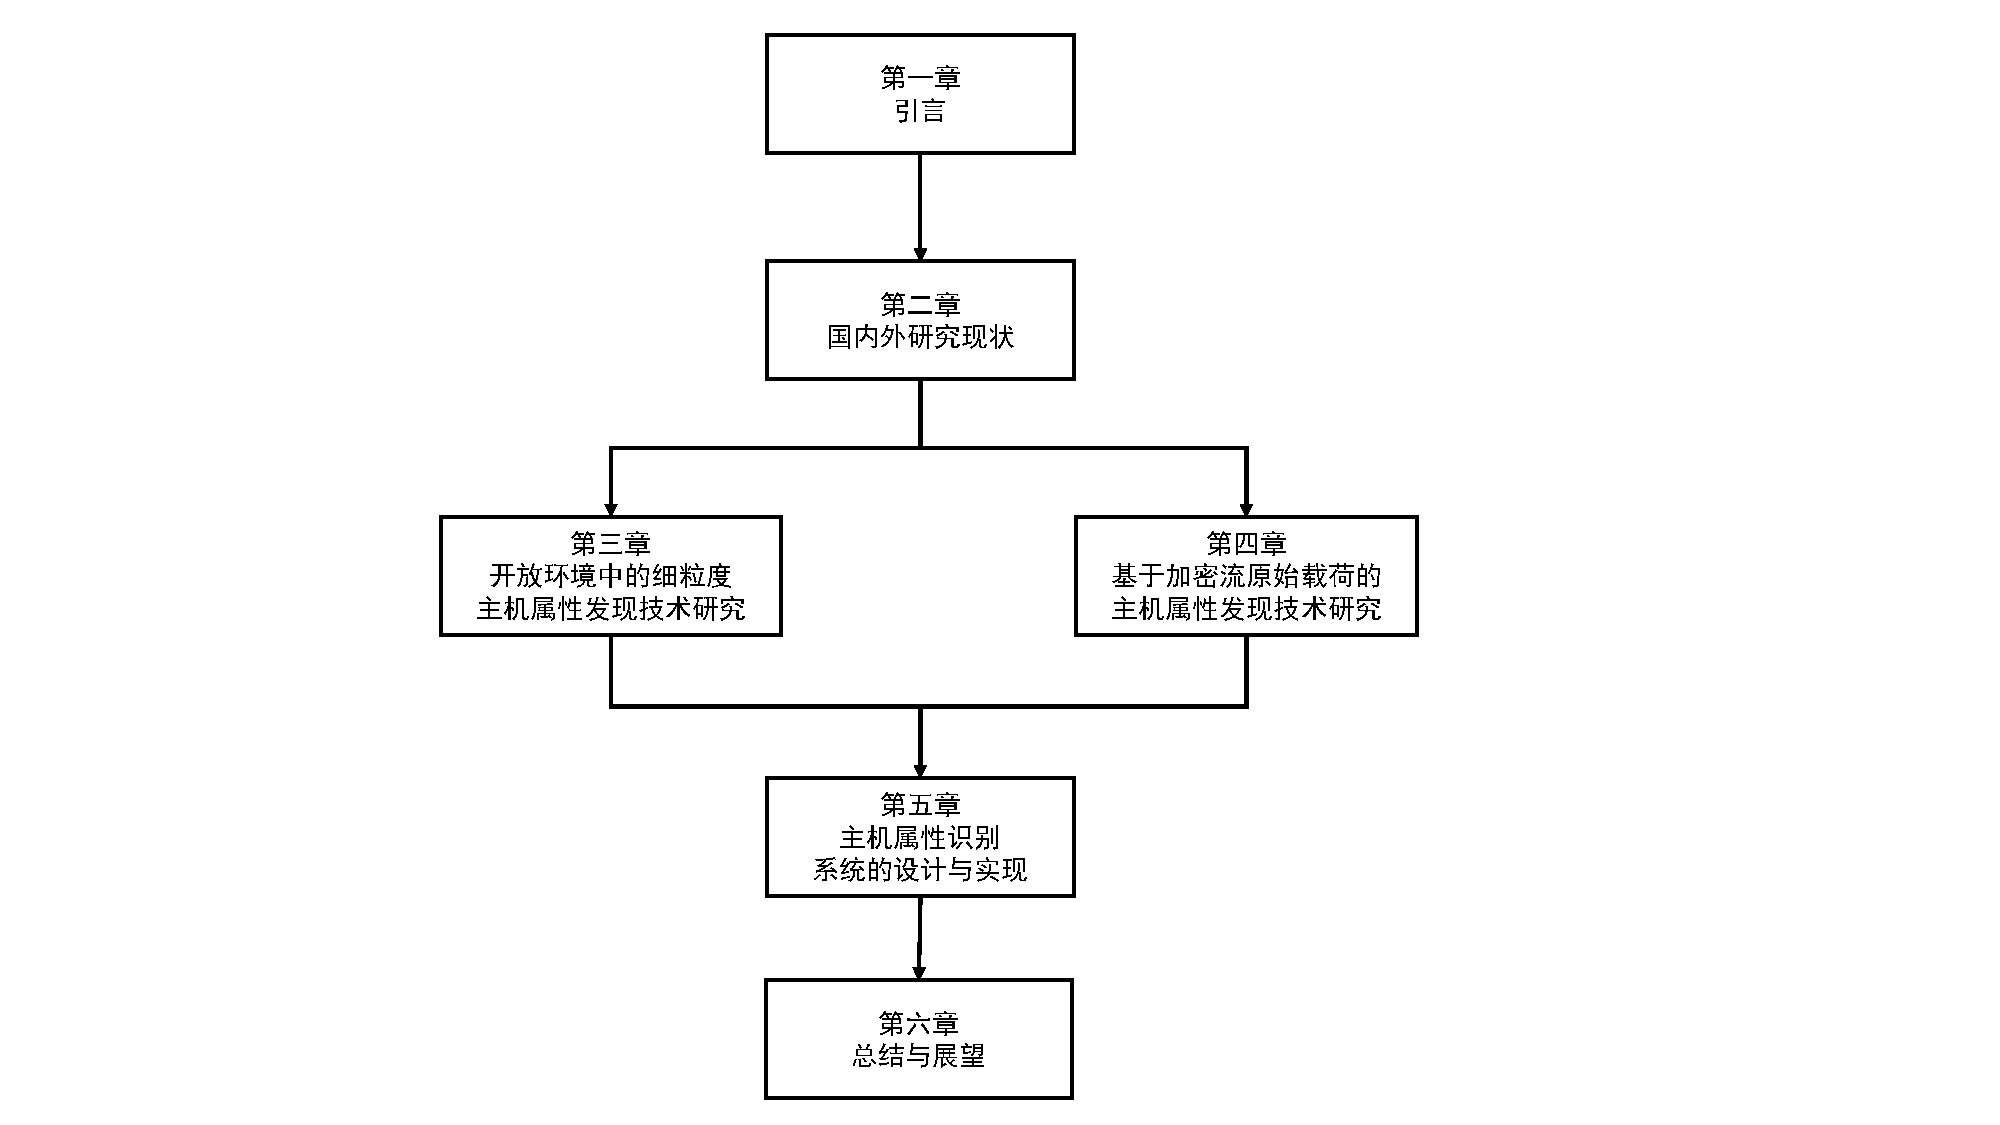
\includegraphics[width=0.8\textwidth]{论文组织结构}
    \bicaption{本文的组织结构}{The structure of this thesis}
\end{figure}

第一章为引言部分,介绍了选题的背景意义、研究内容以及主要贡献,并描述了本文的组织结构。

第二章为国内外研究现状,分别从主动和被动的角度总结了主机属性识别技术的基本原理和研究现状。通过对当前研究成果的总结,发现目前该领域存在的问题,明确本文的研究思路。

第三章为开放环境中的细粒度主机属性发现技术研究,提出了一种基于协议字段特征和流统计特征的主机属性识别方法,着重介绍识别方法的实现细节,包括特征集的选取和机器学习模型效果对比,最终展示识别技术的实验效果。

第四章为基于加密流原始载荷的主机属性发现技术研究,提出了一种利用深度学习模型的主机属性识别方法。此方法基于表示学习的思想,不需要任何先验知识,只需将网络流的原始流数据作为分类器输入,便可完成细粒度的主机属性发现,并拥有更佳的识别效果。

第五章为主机属性识别系统的设计与实现,开发了一套原型系统,可在真实网络中较为准确地识别客户端主机的操作系统类型、版本以及浏览器类型等属性,并具备网络协议识别与解析、TLS流数据属性标注、日志信息存储与查询、主机属性发现实时可视化等功能。

第六章为总结与展望,总结了本文的研究内容与成果,并对未来的研究方向进行了展望。